\documentclass[a4paper, 11pt]{article}
%
\usepackage[utf8]{inputenc}
\usepackage[T1]{fontenc}
\usepackage{lmodern}
\usepackage[francais]{babel}
\usepackage[top=1cm, bottom=1cm, left=1cm, right=2cm]{geometry}
\usepackage{nopageno}
\usepackage{graphicx}
%
\newcommand{\env}[1]{\fbox{\begin{minipage}{\textwidth}#1\end{minipage}}}
%
\title{Exo SD 1 Parenthèses}
\author{Sarfraz \bsc{Kapasi}}
\date{12/02/2013}
%
\begin{document}
%
\maketitle
%
\section{Convertir des schémas de doublets en listes parenthésées}

Convertir sous forme de liste parenthésée simple les schémas doublets de pointeurs ci-dessous.\\

\begin{enumerate}
  \item 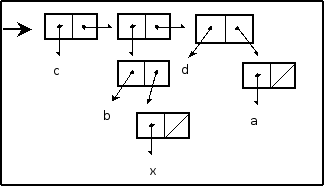
\includegraphics[height=120pt, width=180pt]{Pointeurs_Exo1.png}\\
Réponse: (c (b x) d a)
  \item 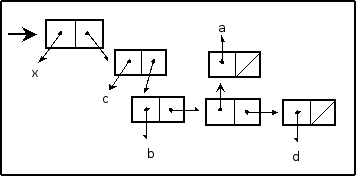
\includegraphics[height=120pt, width=180pt]{Pointeurs_Exo2.png}\\
Réponse: (x c b (a) d)
  \item 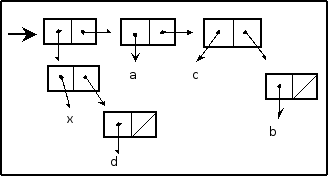
\includegraphics[height=120pt, width=180pt]{Pointeurs_Exo3.png}\\
Réponse: ((x d) a c b)
  \item 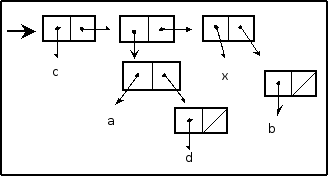
\includegraphics[height=120pt, width=180pt]{Pointeurs_Exo4.png}\\
Réponse: (c (a d) x b)
  \item 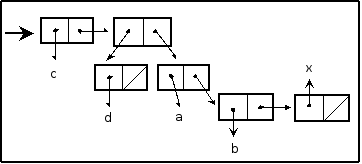
\includegraphics[height=120pt, width=180pt]{Pointeurs_Exo5.png}\\
Réponse: (c (d) a b x)
  \item 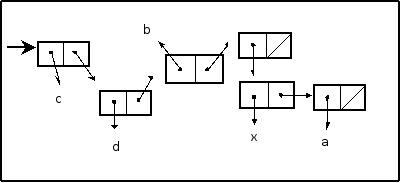
\includegraphics[height=120pt, width=180pt]{Pointeurs_Exo6.png}\\
Réponse: (c d b (x a))
\end{enumerate}

\section{Convertir des listes parenthésées en schémas de doublets}

En vous aidant de l'éditeur de dessins Dia et des schémas de la feuille Lisp spécialement créée pour l'occasion, traduisez en représentation interne (doublets de pointeurs graphiques) les listes suivantes :\\

\begin{enumerate}
    \item (a b x (c d))\\ 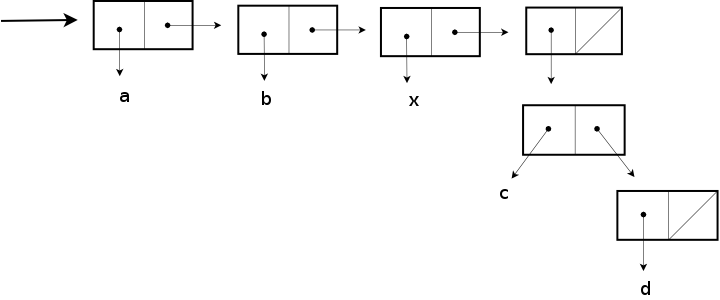
\includegraphics[scale=0.3]{reponse1.png}
    \item ((a) x (b c))\\ 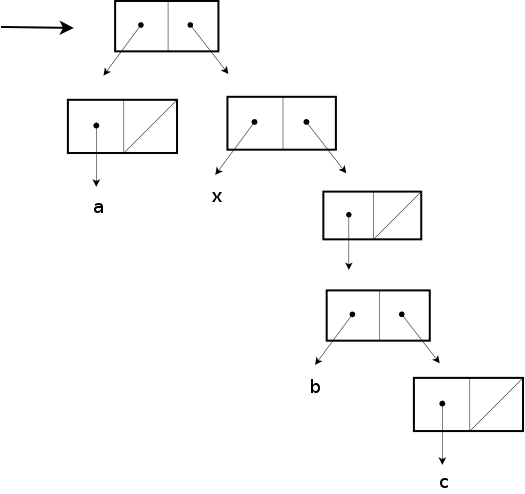
\includegraphics[scale=0.3]{reponse2.png}
    \item (a (b x) c d)\\ 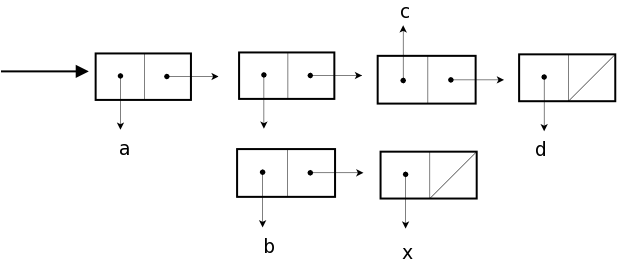
\includegraphics[scale=0.3]{reponse3.png}
    \item (x (b) a (d))\\ 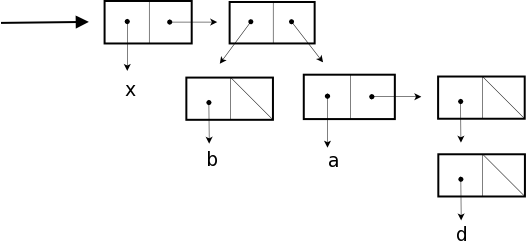
\includegraphics[scale=0.3]{reponse4.png}
    \item ((a b c d x))\\ 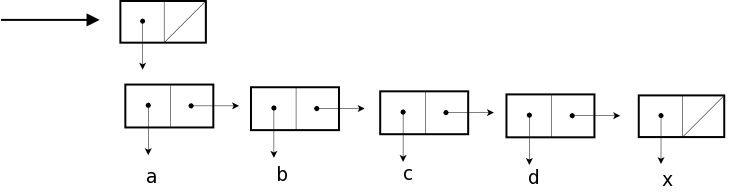
\includegraphics[scale=0.3]{reponse5.png}
    \item (((a)) b c x)\\ 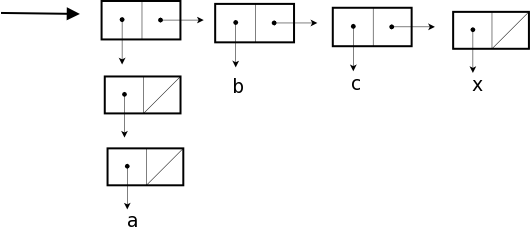
\includegraphics[scale=0.3]{reponse6.png}
\end{enumerate}

%
\end{document}
